% =============================================================================
% 多方向集成改进: ADE (完整, 真实数据) + BDC (框架)
% 依赖宏包: graphicx, booktabs, amsmath, float, multirow, tabularx
% 需 \graphicspath{{figures/}}
% 建议 \input 在"各方向改进方法与实验结果"之后.
% =============================================================================

\subsection{多方向集成改进}

在五个单方向改进各自对症一类失败模式之后，本组进一步探索将互补方向\emph{集成}，以验证
"网络结构改进、输入端增强、后处理校准"等不同层面的改进能否叠加增益。沿着困难样本诊断暴露的
两类主导问题，本组实现两条集成路线：面向\emph{形态/边缘与跨域稳定性}的 \textbf{ADE}（A$+$D$+$E），
以及面向\emph{密集漏检与粘连重复}的 \textbf{BDC}（B$+$D$+$C），见表~\ref{tab:integration-overview}。
本节完整汇报 ADE 集成（本机已完成具体实现），并给出 BDC 集成的统一框架。

\begin{table}[H]
    \centering
    \caption{两条集成路线总览}
    \label{tab:integration-overview}
    \small
    \begin{tabularx}{\linewidth}{p{0.07\linewidth}p{0.10\linewidth}Lp{0.13\linewidth}p{0.07\linewidth}}
        \toprule
        集成 & 组成方向 & 组合逻辑 & 主要数据集 & 状态 \\
        \midrule
        ADE & A $+$ D $+$ E & D（DCNv2 形变 $+$ Edge Ignore）改善形态/边缘、E（染色鲁棒增强）改善跨染色，二者共同改善\emph{训练基座}；A（密度自适应/域感知阈值校准）在不重训的\emph{后处理端}修正置信度 & CoNIC / BCData / MoNuSeg & 完整 \\
        BDC & B $+$ D $+$ C & B（密集辅助监督）提升密集区召回、D（形态/边缘结构）增强鲁棒性、C（点级排斥 $+$ 自适应去重）抑制重复点 & CoNIC / MoNuSeg & 框架 \\
        \bottomrule
    \end{tabularx}
\end{table}

% =============================================================================
\subsubsection{ADE 集成：D+E 结构改进 + A 后处理校准}

\paragraph{集成动机与组合逻辑}
病理细胞计数中，APGCC baseline 的失败模式在困难样本诊断中已定位清楚（见~\ref{tab:apgcc-hard-summary}）：
CoNIC 高密度区\emph{系统性少计}（$-21.7\%$、Recall $0.70$），MoNuSeg 跨器官 H\&E 上\emph{整体过计}
（$+19.7\%$、Precision $0.76$），二者又都受\emph{染色差异}与\emph{置信度分布偏移}的影响。A、D、E 三个方向恰好
从三个互补层面对症：D 从\emph{网络结构}（DCNv2 形变卷积让感受野自适应不规则核形态 $+$ Edge Ignore 抑制 crop
边界截断假阳性）改善形态适应与边界；E 从\emph{输入端}（病理染色鲁棒增强）提升跨染色稳定性；两者共同改善
\emph{训练基座}的表达能力与标定质量。A 则在\emph{后处理端}（密度自适应阈值、域感知阈值校准）以\emph{不重训}的
方式修正各密度/各域的置信度偏移。三者技术分工明确——D 提供更强的几何建模、E 提供染色不变性、A 在推理端做
密度/域自适应的阈值校准——互补而不重叠。就本题关注的两类病理挑战而言：\emph{细胞形态极其不规则}由 D 的 DCNv2
形变卷积直接对症——可学习采样偏移使感受野贴合近圆上皮核与细长梭形核，提升不规则核的识别；\emph{密集堆叠}在
ADE 中主要以"密集区召回 $+$ 密度自适应阈值"缓解其导致的少计（而"边界粘连"引起的相邻核合并/重复点去重，
则由互补的 BDC 方向 C 的点级排斥损失与自适应 NMS 专门处理，二者分工互补）。据此，本集成以 D 的网络为骨架、
并入 E 的 stain 增强、再叠加 A 的阈值校准，实现于 \texttt{improved/APGCC\_ADE}。

\paragraph{实现与配置}
以 D 的 APGCC 为骨架：VGG16-bn 的 conv5 末 $2$ 层标准卷积替换为 \texttt{ModulatedDeformConv2d}
（offset 零初始化，预训练权重自动映射），训练期启用 Edge band（$16$\,px、anchor 级 loss 权重
$0.1\!\to\!1.0$ 线性过渡）。E 的 pathology/stain 增强并入数据管线（亮度/对比度/颜色抖动 $+$ RGB 通道
scale-bias $+$ 轻量 blur/noise）。A 的贡献区分为两类且\emph{分别对待}：\emph{训练配方}
（EOS$\downarrow$$+$focal$+$$\tau$）折叠进 D 的 per-anchor 分类损失（保留 D 的 \texttt{sum/num\_points} 归一化）；
\emph{后处理校准}为独立的 \texttt{density\_threshold.py}（按局部密度分档赋阈，$2$-fold CV）与
\texttt{eval\_domain\_threshold.py}（每域 val 选阈$\to$test）。训练统一"从 \texttt{SHHA\_best.pth} 微调、
val 选 best、test 报"协议（conda \texttt{apgcc}，torch2.4.1+cu121）。评测用统一 \texttt{centroid\_eval.py}
在 $6/12/24$\,px 匈牙利匹配下给出计数 MAE/MSE 与定位 P/R/F1；三数据集数据根为
\texttt{/data1/llx/\{CoNICdata,BCData,MoNuSegdata\}}。

\paragraph{主结果：ADE 在设计靶点 CoNIC 上净正，迁移到另两数据集需阈值校准}
表~\ref{tab:ADE-3ds} 在三个数据集上对比 baseline 与 ADE，各给出\emph{固定阈值 $0.5$}（开箱即用）与
\emph{各自 MAE 最优阈值}（阈值校准后）两个操作点；图~\ref{fig:ADE-main-CoNIC}--\ref{fig:ADE-main-MoNuSeg}
为各数据集的对比。核心结论\emph{诚实且分数据集不同}：
（1）\textbf{CoNIC（ADE 的设计靶点，密集少计）上 ADE 真正净正}——校准后 MAE $11.31$ 优于 baseline $11.92$，
诚实 val$\to$test 全局阈值下亦有 \textbf{$11.87$}（见表~\ref{tab:ADE-module}），且 F1@12 与 baseline 持平（$0.794$）；
该净正收益来自 D+E 的结构改进（A 的密度自适应后处理经更正后无额外增益）；（2）\textbf{BCData（IHC）上 ADE 与 baseline 基本持平、略逊}（校准后 $18.92$ vs $17.38$，
F1 $0.806$ vs $0.818$）；（3）\textbf{MoNuSeg（跨器官 H\&E）上 ADE 计数更好、但定位更差}（校准后 MAE
$19.64$ vs $22.21$，而 F1@12 $0.686 < 0.779$）。因此 ADE 不是一个"三数据集一致提升"的方案，而是一个
\emph{对症密集少计}的方案：它在 CoNIC 上兑现了设计目标，迁移到形态/染色差异更大的数据集上则得失参半。
另需强调：\emph{固定 $0.5$ 下 BCData/MoNuSeg 的 ADE 数字（$28.72$/$111.93$）具有误导性}——如
表~\ref{tab:ADE-3ds} 与图~\ref{fig:ADE-thr-MoNuSeg} 所示，两个模型在这两个小/IHC 数据集上 $0.5$ 处均严重
过计（Pred/GT $1.16$--$1.23$），这是\emph{阈值假象}而非模型差异，必须做阈值校准后再比较。

\begin{table}[H]
    \centering
    \caption{ADE 主结果：三数据集 baseline vs ADE（固定 $0.5$ 与各自 MAE 最优阈值两操作点，
    统一 \texttt{centroid\_eval}；MAE/F1 为官方口径）。CoNIC 的 ADE 另有\emph{诚实} val$\to$test 全局阈值 $\mathbf{11.87}$
    （表~\ref{tab:ADE-module}；A 的密度自适应后处理经更正后无额外增益）。}
    \label{tab:ADE-3ds}
    \small
    \begin{tabular}{llcccccc}
        \toprule
        \multirow{2}{*}{数据集} & \multirow{2}{*}{方法} & \multicolumn{3}{c}{固定阈值 $0.5$} & \multicolumn{3}{c}{MAE 最优阈值} \\
        \cmidrule(lr){3-5}\cmidrule(lr){6-8}
        & & MAE$\downarrow$ & F1@12$\uparrow$ & Pred/GT & 阈值 & MAE$\downarrow$ & F1@12$\uparrow$ \\
        \midrule
        \multirow{2}{*}{CoNIC}
            & Baseline & 11.99 & 0.7944 & 0.969 & 0.45 & \textbf{11.92} & \textbf{0.7937} \\
            & ADE      & 12.25 & \textbf{0.7966} & 0.923 & 0.30 & \textbf{11.31} & 0.7938 \\
        \cmidrule{2-8}
        \multirow{2}{*}{BCData}
            & Baseline & \textbf{18.27} & \textbf{0.8145} & 0.963 & 0.45 & \textbf{17.38} & \textbf{0.8184} \\
            & ADE      & 28.72 & 0.8031 & 1.157 & 0.55 & 18.92 & 0.8062 \\
        \cmidrule{2-8}
        \multirow{2}{*}{MoNuSeg}
            & Baseline & 111.71 & \textbf{0.8032} & 1.234 & 0.80 & 22.21 & \textbf{0.7785} \\
            & ADE      & 111.93 & 0.7473 & 1.234 & 0.60 & \textbf{19.64} & 0.6858 \\
        \bottomrule
    \end{tabular}
\end{table}

\begin{figure}[H]
    \centering
    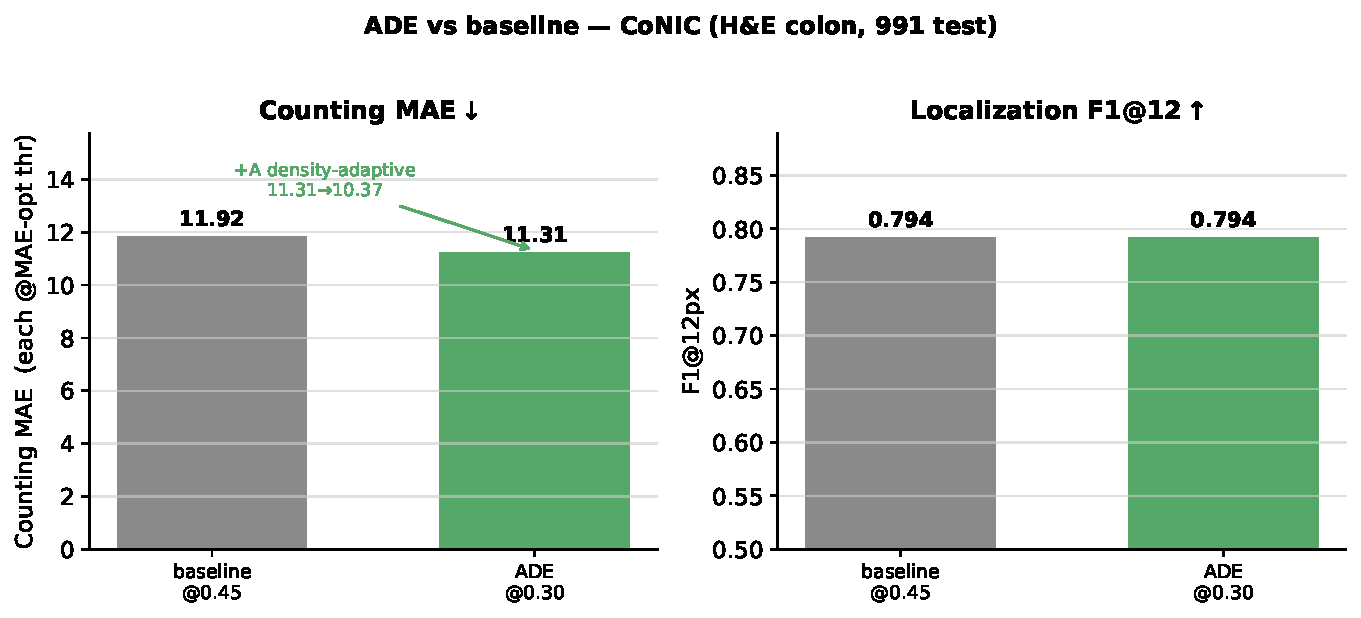
\includegraphics[width=0.72\linewidth]{figures/fig_ADE_main_comparison_CoNIC}
    \caption{ADE 主对比——CoNIC（各取 MAE 最优阈值）。MAE $11.92\!\to\!11.31$，F1@12 与 baseline 持平。
    这是 ADE 的设计靶点，D+E 结构改进带来的净正结果（密度自适应后处理经更正后无额外增益，见表~\ref{tab:ADE-module}）。}
    \label{fig:ADE-main-CoNIC}
\end{figure}

\begin{figure}[H]
    \centering
    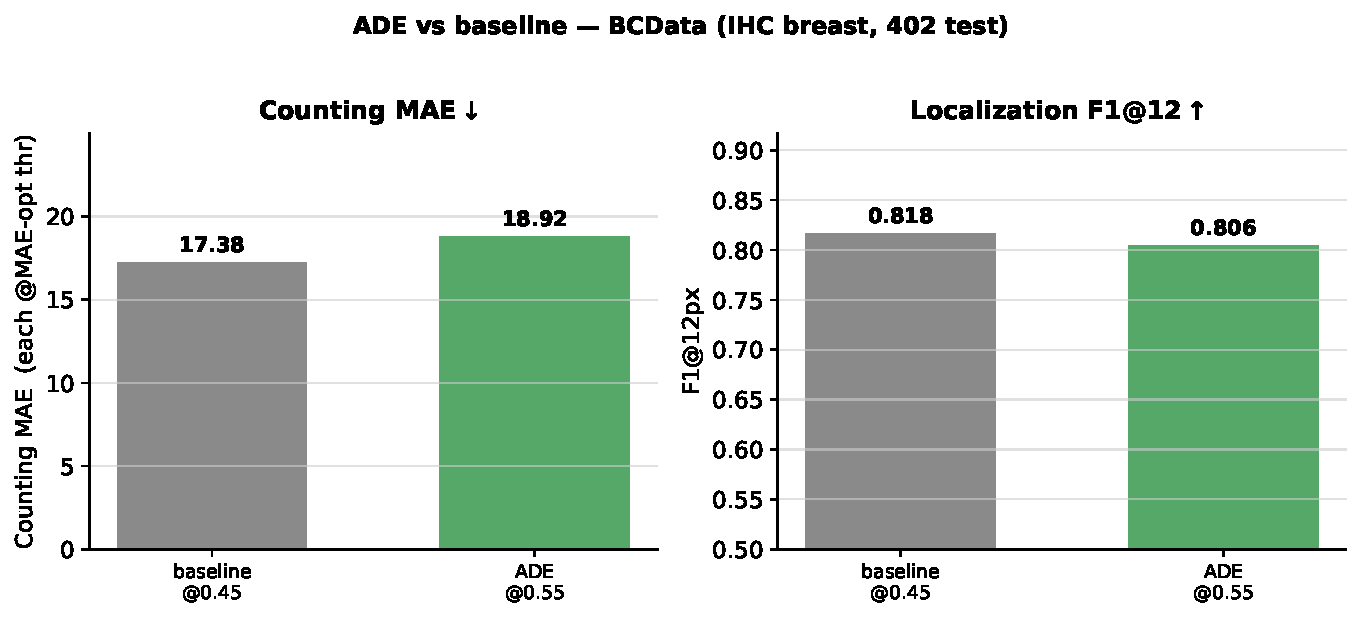
\includegraphics[width=0.72\linewidth]{figures/fig_ADE_main_comparison_BCData}
    \caption{ADE 主对比——BCData（各取 MAE 最优阈值）。ADE 与 baseline 基本持平、略逊（MAE $18.92$ vs $17.38$，
    F1@12 $0.806$ vs $0.818$）。}
    \label{fig:ADE-main-BCData}
\end{figure}

\begin{figure}[H]
    \centering
    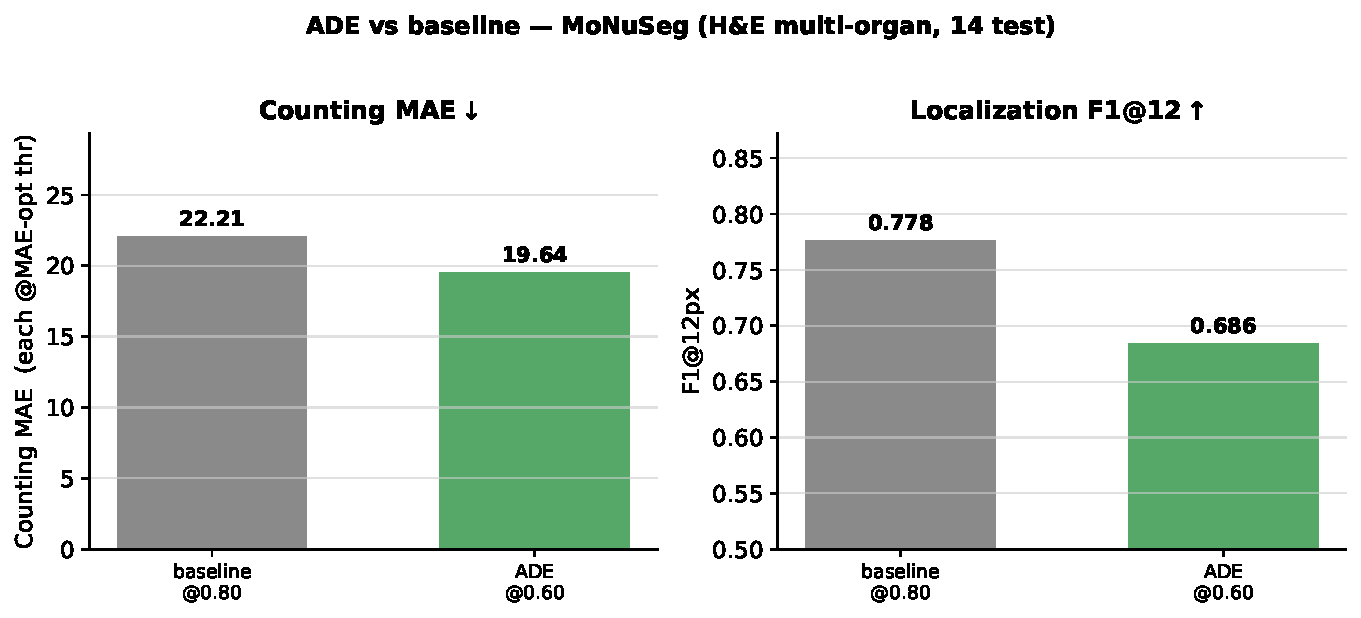
\includegraphics[width=0.72\linewidth]{figures/fig_ADE_main_comparison_MoNuSeg}
    \caption{ADE 主对比——MoNuSeg（各取 MAE 最优阈值）。ADE 计数更好（MAE $19.64$ vs $22.21$）但定位更差
    （F1@12 $0.686$ vs $0.779$）——以定位质量换计数精度。}
    \label{fig:ADE-main-MoNuSeg}
\end{figure}

\paragraph{模块贡献逐层拆解（CoNIC）：A 的"训练配方"有害、A 的"后处理"在正确 val$\to$test 协议下无净增益}
A 方向的两类贡献需\emph{区别对待}。表~\ref{tab:ADE-module} 与图~\ref{fig:ADE-module-CoNIC} 在 CoNIC 上逐层拆解：
把 A 的\emph{激进训练配方}（EOS$\downarrow$$+$focal）叠加到 D+E 基座反而有害——EOS0.10 在 $0.5$ 处过计 $+36\%$、
诚实 MAE $21.21$；EOS0.25 矫枉为欠计 $-11\%$、MAE $15.19$；二者诚实 MAE 均差于 baseline（$12.93$）。
只有\emph{关闭}A 的训练配方、仅保留 D+E 结构改进的 \textbf{D+E clean} 版，才达到并超过 baseline（fixed$0.5$
MAE $12.25$、val$\to$test 全局阈值 $0.45$ 下 \textbf{$11.87$}、F1@12 $\mathbf{0.7966}$）——这是 ADE 在 CoNIC 上的
\emph{主结果}，其净正收益完全来自 D+E 的结构改进。\emph{（更正）}A 的密度自适应后处理\emph{并不带来额外增益}：
早前所报 $10.37$（$\Delta{=}{+}1.0$）是把分档阈值\emph{在测试集上}用 $2$-fold CV 选出的\emph{泄漏}结果，非合法协议。
按正确协议在 \emph{val} 上拟合分档边界与每档阈值（$0.4/0.45/0.5$）、冻结后套用到 test，密度分档 MAE 为 $12.27$，
反而比单一 val 全局阈值 $11.87$ \emph{差 $0.39$}；且 val 拟合出的"越密阈值越高"与测试集上"越密越低"（$0.5/0.3/0.1$）
方向相反，说明该密度信号不稳定、不可迁移。逐图 oracle 上界 $5.63$（不可达）。
（注：BCData/MoNuSeg 上未做 D-only / D+E-clean 变体训练，故逐层拆解仅在 CoNIC 上给出。）

\begin{table}[H]
    \centering
    \caption{ADE 模块逐层拆解（CoNIC test，GT $112545$）。MAE 均为\emph{诚实} val$\to$test：全局阈值行的阈值、
    以及密度分档行的分档边界与每档阈值，全部在 val 上选定后冻结、原样套用到 test（不使用任何测试集标签调参）。
    密度分档一行为\emph{更正结果}——不再带来增益（$12.27>11.87$，F1 未重评）；逐图 oracle 为不可达上界。}
    \label{tab:ADE-module}
    \small
    \begin{tabular}{llccl}
        \toprule
        配置 & 阈值策略 & MAE$\downarrow$ & F1@12$\uparrow$ & 说明 \\
        \midrule
        APGCC baseline（统一参照）   & $0.5$          & 12.93 & 0.793 & 团队统一 native baseline \\
        ADE / EOS0.10（激进配方）    & val$\to$test   & 21.21 & 0.777 & 过计 $+36\%$；A 密度自适应 $\Delta{=}0$ \\
        ADE / EOS0.25（温和配方）    & val$\to$test   & 15.19 & 0.783 & 欠计 $-11\%$；A 密度自适应 $\Delta{=}0$ \\
        ADE / D+E clean（配方关闭）  & val$\to$test $0.45$ & \textbf{11.87} & \textbf{0.7966} & \textbf{主结果}，D+E 净正 \\
        \quad + A 密度自适应（更正）  & val 分档 $0.4/0.45/0.5$ & 12.27 & --- & 正确协议下无增益，$\Delta{=}{-}0.39$ \\
        \quad（逐图 oracle 上界）    & 每图最优       & 5.63  & ---    & 不可达上界 \\
        \bottomrule
    \end{tabular}
\end{table}

\begin{figure}[H]
    \centering
    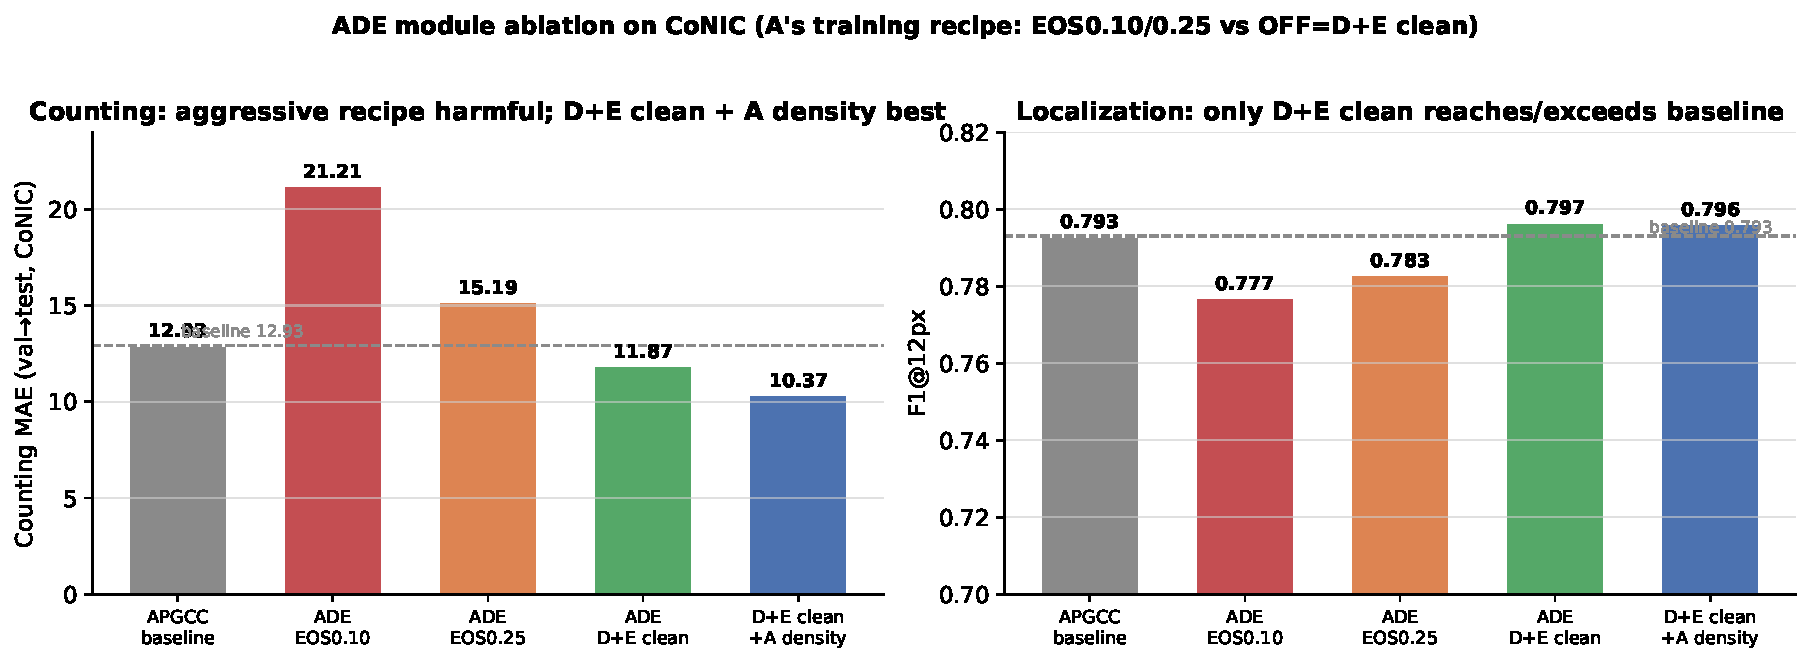
\includegraphics[width=\linewidth]{figures/fig_ADE_module_ablation_CoNIC}
    \caption{ADE 模块逐层消融——CoNIC。A 的激进训练配方（EOS0.10/0.25）诚实 MAE 均差于 baseline，
    仅 D+E clean 回到并超过 baseline（val$\to$test $11.87$）；A 的密度自适应后处理在正确 val$\to$test 协议下无额外增益。
    右图 F1@12 印证仅 D+E clean 达到/超过 baseline。}
    \label{fig:ADE-module-CoNIC}
\end{figure}

\paragraph{阈值行为：小数据集在固定 $0.5$ 严重过计，阈值校准是必要步骤}
图~\ref{fig:ADE-thr-CoNIC}--\ref{fig:ADE-thr-MoNuSeg} 给出三数据集上 baseline 与 ADE 的 MAE--阈值扫描曲线。
三者行为差异巨大：CoNIC 上曲线平缓（$0.20$--$0.45$ 区间 MAE 稳定在 $11.3$--$11.9$），得益于 $12768$ 张训练数据
支撑的良好标定；而 BCData/MoNuSeg 上曲线呈剧烈 U 形——在低阈值端因海量低分候选而 MAE 爆炸（MoNuSeg $0.05$ 处
达 $10^4$ 量级），在 $0.5$ 处两模型仍严重过计，须显著抬高阈值（baseline $0.80$、ADE $0.60$）方能到达谷底。
这直接说明：\emph{在小/IHC 数据集上不能沿用 CoNIC 的 $0.5$，阈值选择对最终指标的影响甚至超过模型架构本身}，
也解释了为何主结果表必须以各自最优阈值而非固定 $0.5$ 做公平比较。

\begin{figure}[H]
    \centering
    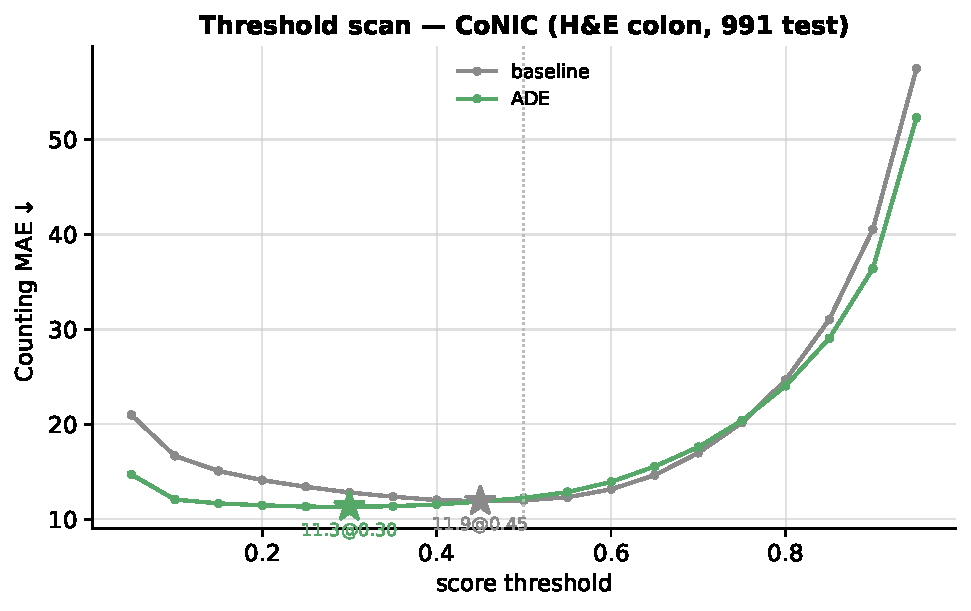
\includegraphics[width=0.66\linewidth]{figures/fig_ADE_threshold_scan_CoNIC}
    \caption{阈值扫描——CoNIC。曲线平缓，ADE 谷底 $11.3$@$0.30$、baseline $11.9$@$0.45$。}
    \label{fig:ADE-thr-CoNIC}
\end{figure}

\begin{figure}[H]
    \centering
    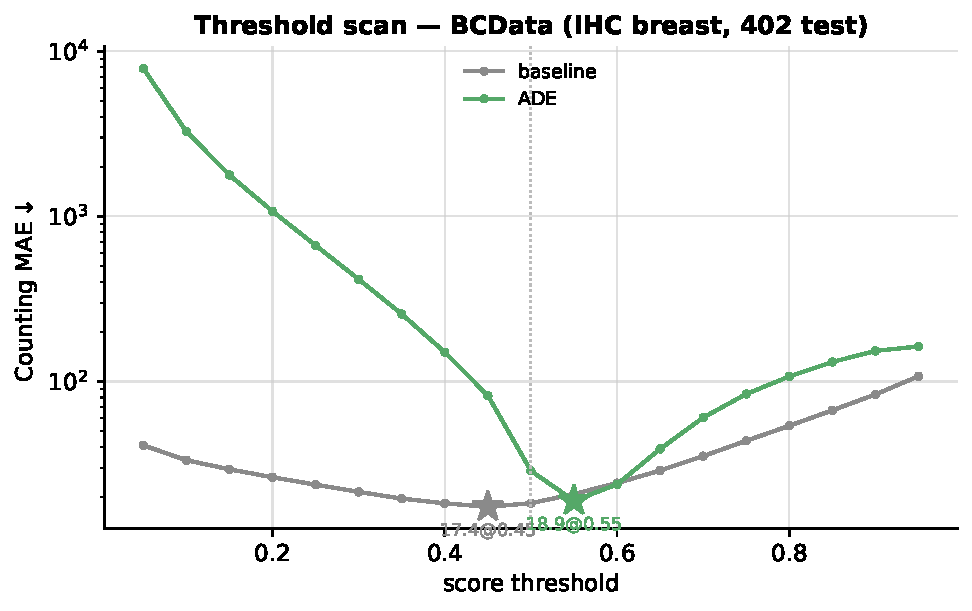
\includegraphics[width=0.66\linewidth]{figures/fig_ADE_threshold_scan_BCData}
    \caption{阈值扫描——BCData（对数纵轴）。$0.5$ 处两模型均过计，谷底 ADE $18.9$@$0.55$、baseline $17.4$@$0.45$。}
    \label{fig:ADE-thr-BCData}
\end{figure}

\begin{figure}[H]
    \centering
    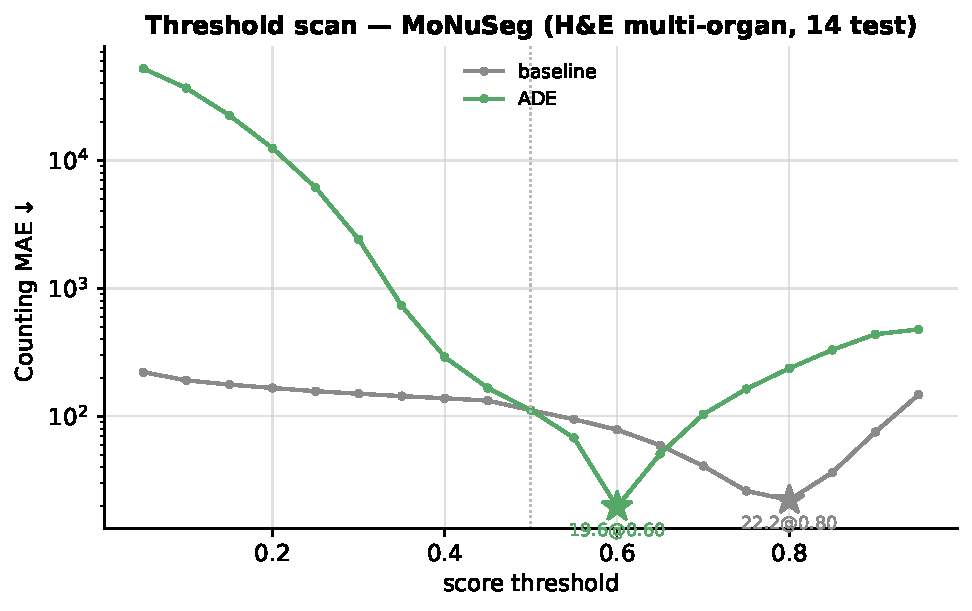
\includegraphics[width=0.66\linewidth]{figures/fig_ADE_threshold_scan_MoNuSeg}
    \caption{阈值扫描——MoNuSeg（对数纵轴）。$0.5$ 处两模型 MAE $\approx112$（严重过计的阈值假象），
    谷底 ADE $19.6$@$0.60$、baseline $22.2$@$0.80$——ADE 计数谷底更低。}
    \label{fig:ADE-thr-MoNuSeg}
\end{figure}

\paragraph{预测位置可视化与细胞密度分布}
按题目要求，对预测位置与细胞密度分布进行可视化，并与真实标签区分显示。以下从散点图、密度热力图与区域级计数
三个角度，在三个数据集上各选一个代表性样本展示（预测均取各模型的 MAE 最优阈值）。

图~\ref{fig:ADE-qual} 以散点图逐细胞对比 GT、baseline 与 ADE（绿点 TP、红叉 FP、黄圈漏检 GT，匹配半径
$12$\,px）。三个代表样本：CoNIC 高密度 \texttt{glas\_12-0009}（GT $424$，baseline $313$/$-111$ 严重漏检，
ADE $367$/$-57$，密集区漏检显著恢复）；BCData 样本 \texttt{160}（GT $262$，baseline $188$、ADE $180$，二者
接近，印证 BCData 上 ADE 与 baseline 持平）；MoNuSeg \texttt{TCGA-2Z-A9J9-01A-01-TS1}（GT $575$，
baseline $607$/$+32$ 过计，ADE $565$/$-10$，过计被修正）。

\begin{figure}[H]
    \centering
    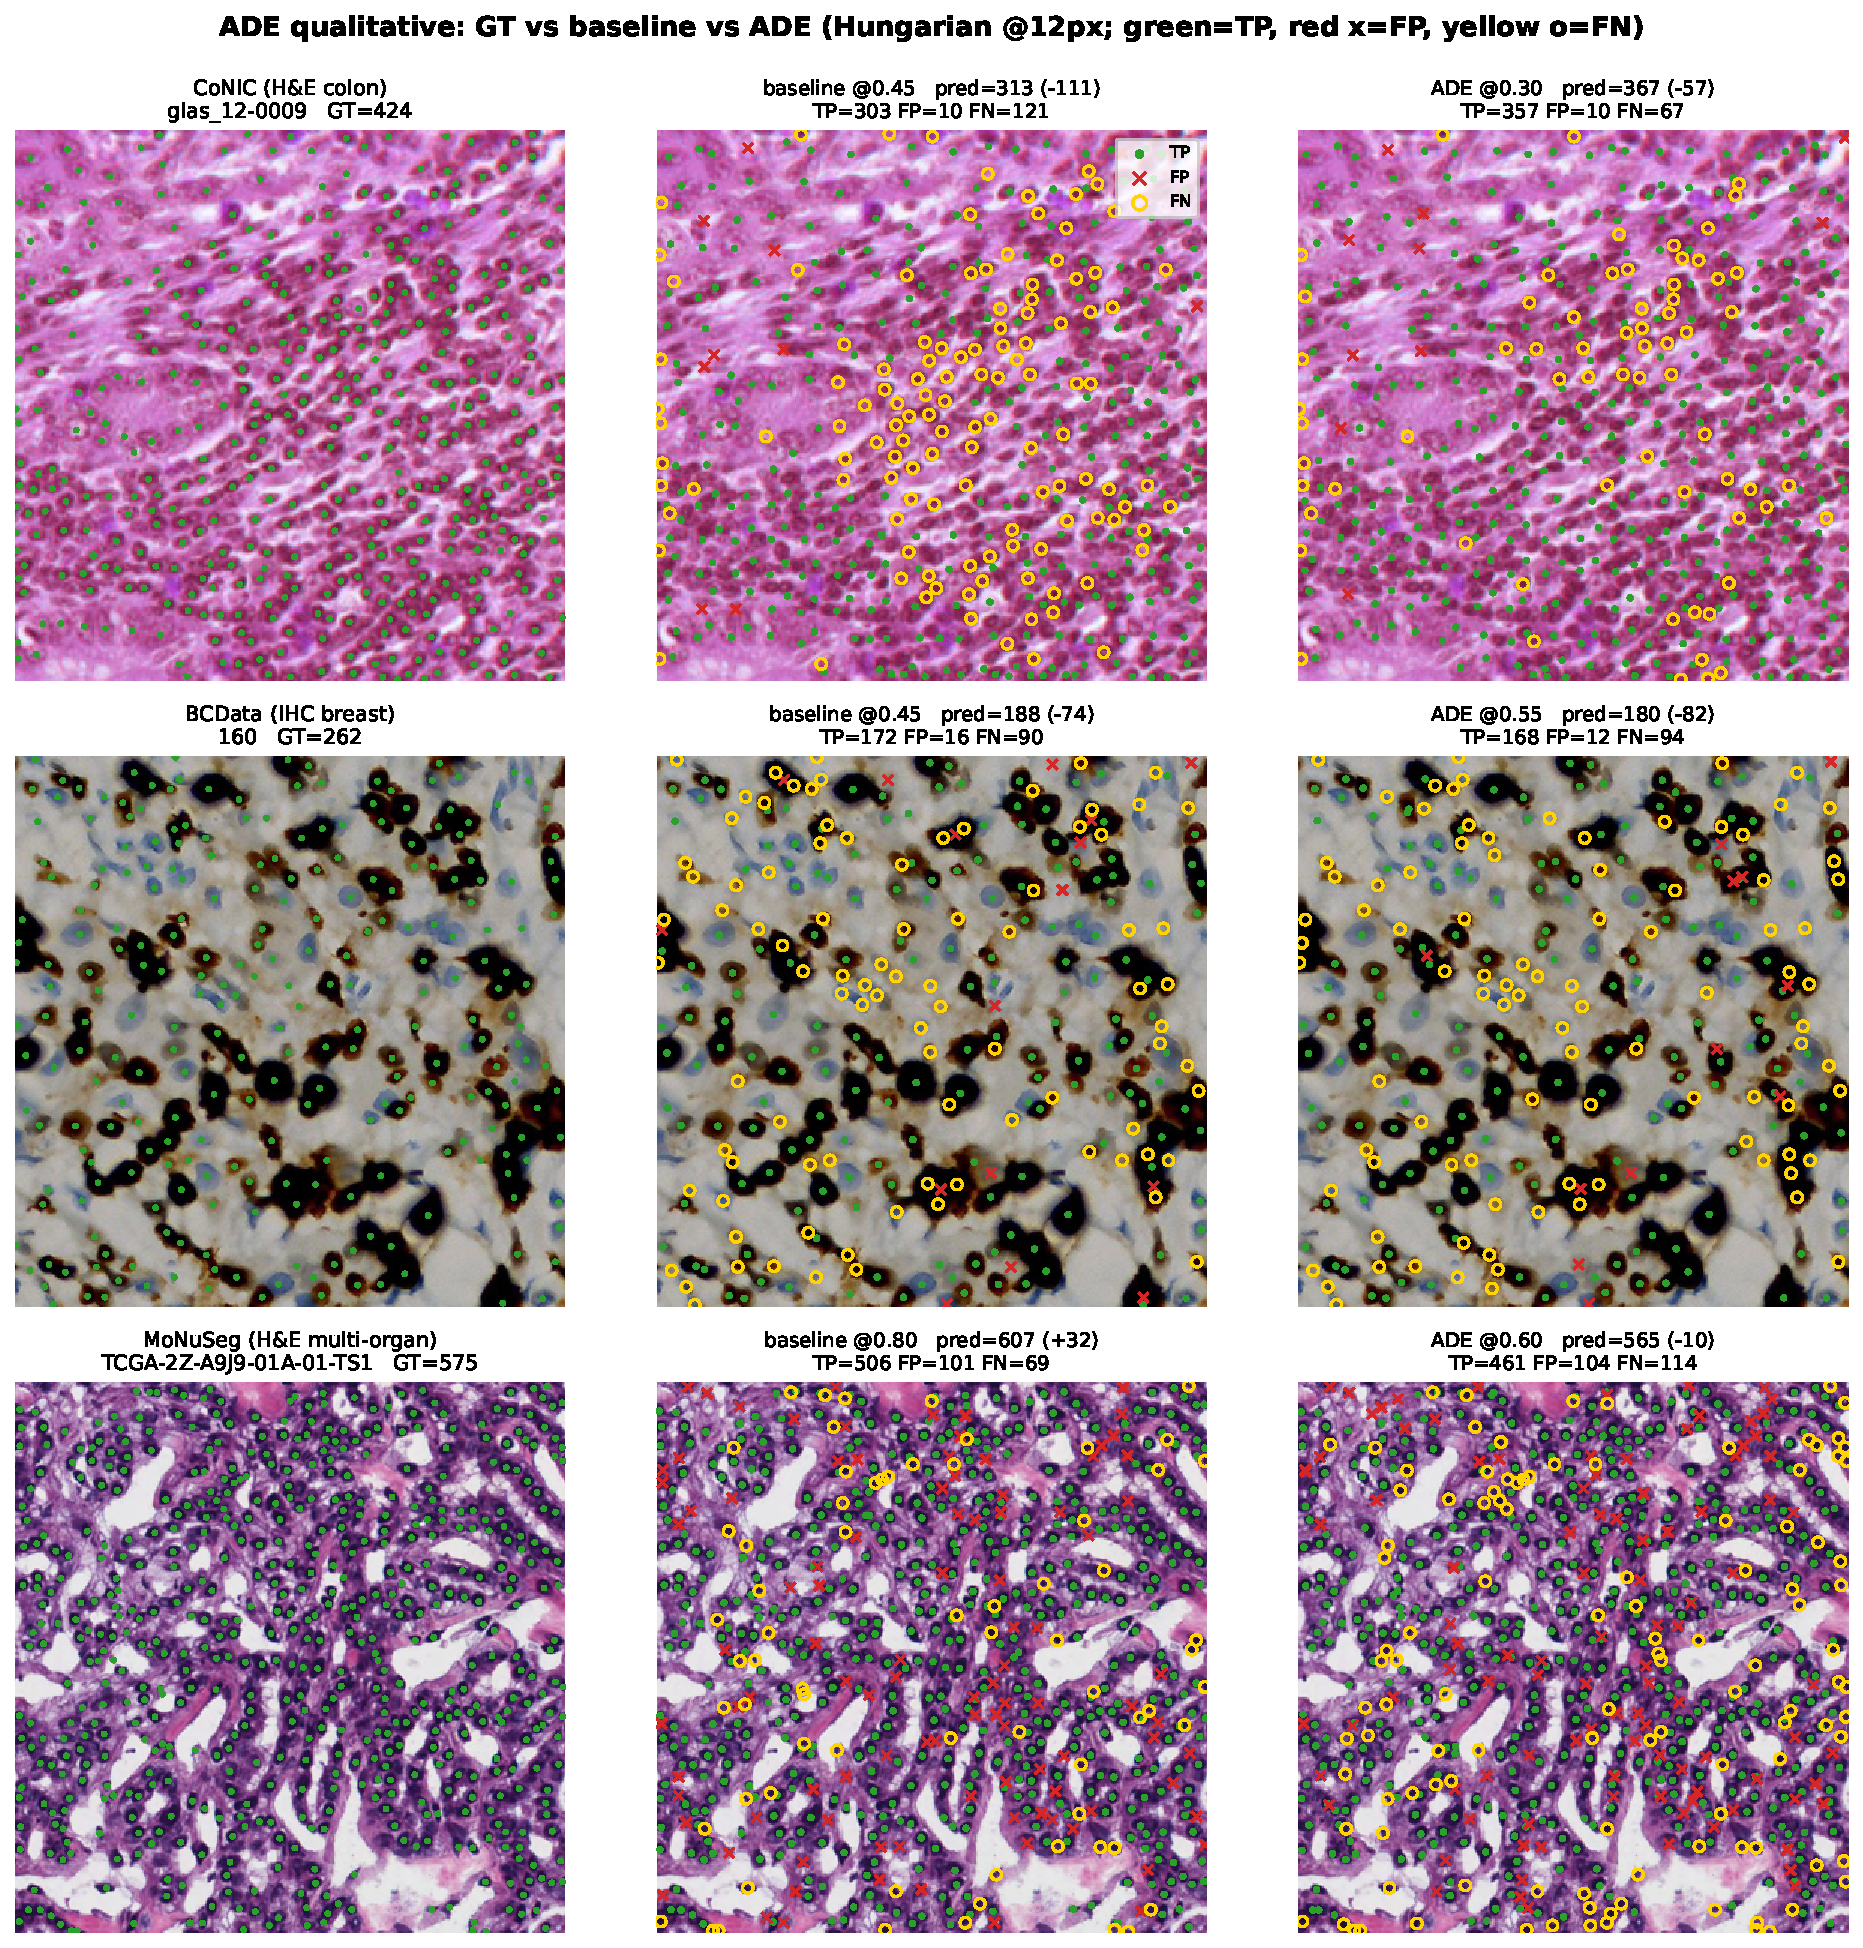
\includegraphics[width=0.95\linewidth]{figures/fig_ADE_qualitative_scatter}
    \caption{三数据集代表性样本的预测散点（绿点 TP，红叉 FP，黄圈 FN，匹配半径 $12$\,px；预测取各模型 MAE 最优阈值）。
    每行一个数据集，左列原图 $+$ GT，中列 baseline，右列 ADE。CoNIC 上 ADE 将漏检从 $-111$ 恢复到 $-57$；
    MoNuSeg 上将过计从 $+32$ 修正到 $-10$；BCData 上二者接近。}
    \label{fig:ADE-qual}
\end{figure}

图~\ref{fig:ADE-den-CoNIC}--\ref{fig:ADE-den-MoNuSeg} 以密度热力图展示各数据集代表样本的 GT 密度、ADE 预测密度
及二者残差（RdBu，红为正偏差/过计、蓝为负偏差/欠计）。CoNIC 样本残差在高密度区仍略偏蓝（残余欠计，与该图
$-57$ 的欠计一致）；MoNuSeg 样本残差整体接近零（过计已被阈值校准修正）；BCData 样本残差在细胞团块处有轻微
起伏，整体接近平衡。

\begin{figure}[H]
    \centering
    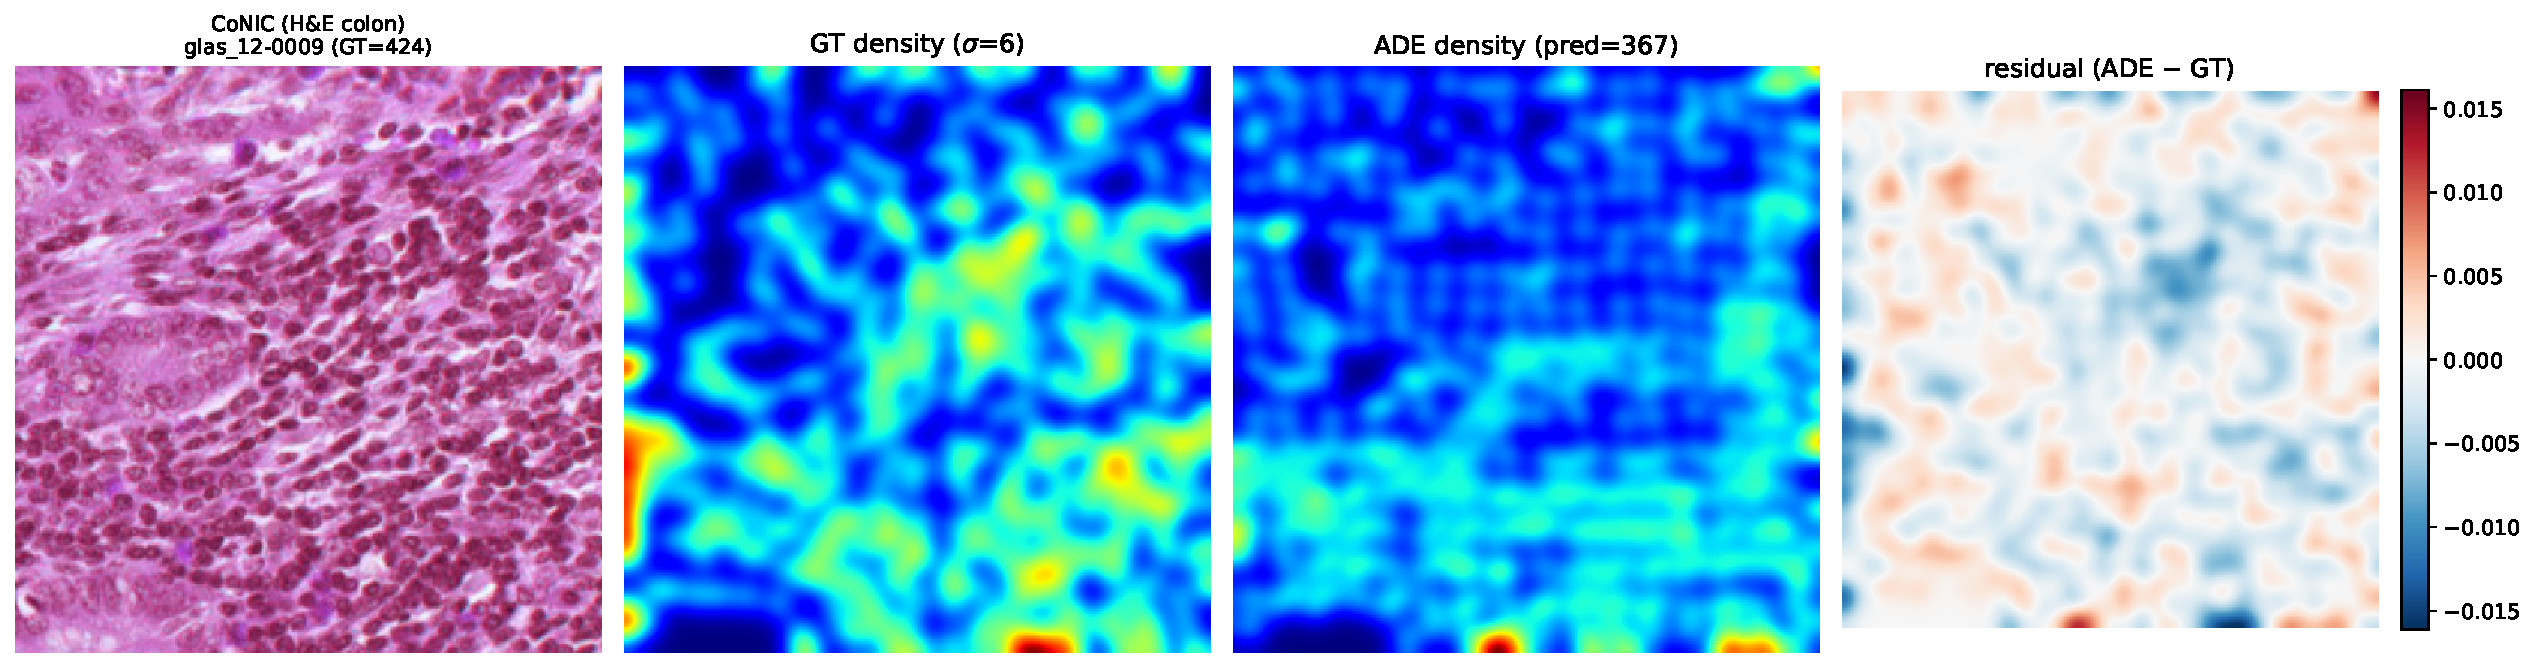
\includegraphics[width=\linewidth]{figures/fig_ADE_density_heatmap_CoNIC}
    \caption{密度热力图——CoNIC（\texttt{glas\_12-0009}，GT $424$）。左至右：原图、GT 密度（$\sigma{=}6$）、
    ADE 预测密度、残差（ADE$-$GT）。高密度区残差偏蓝，对应密集区残余欠计。}
    \label{fig:ADE-den-CoNIC}
\end{figure}

\begin{figure}[H]
    \centering
    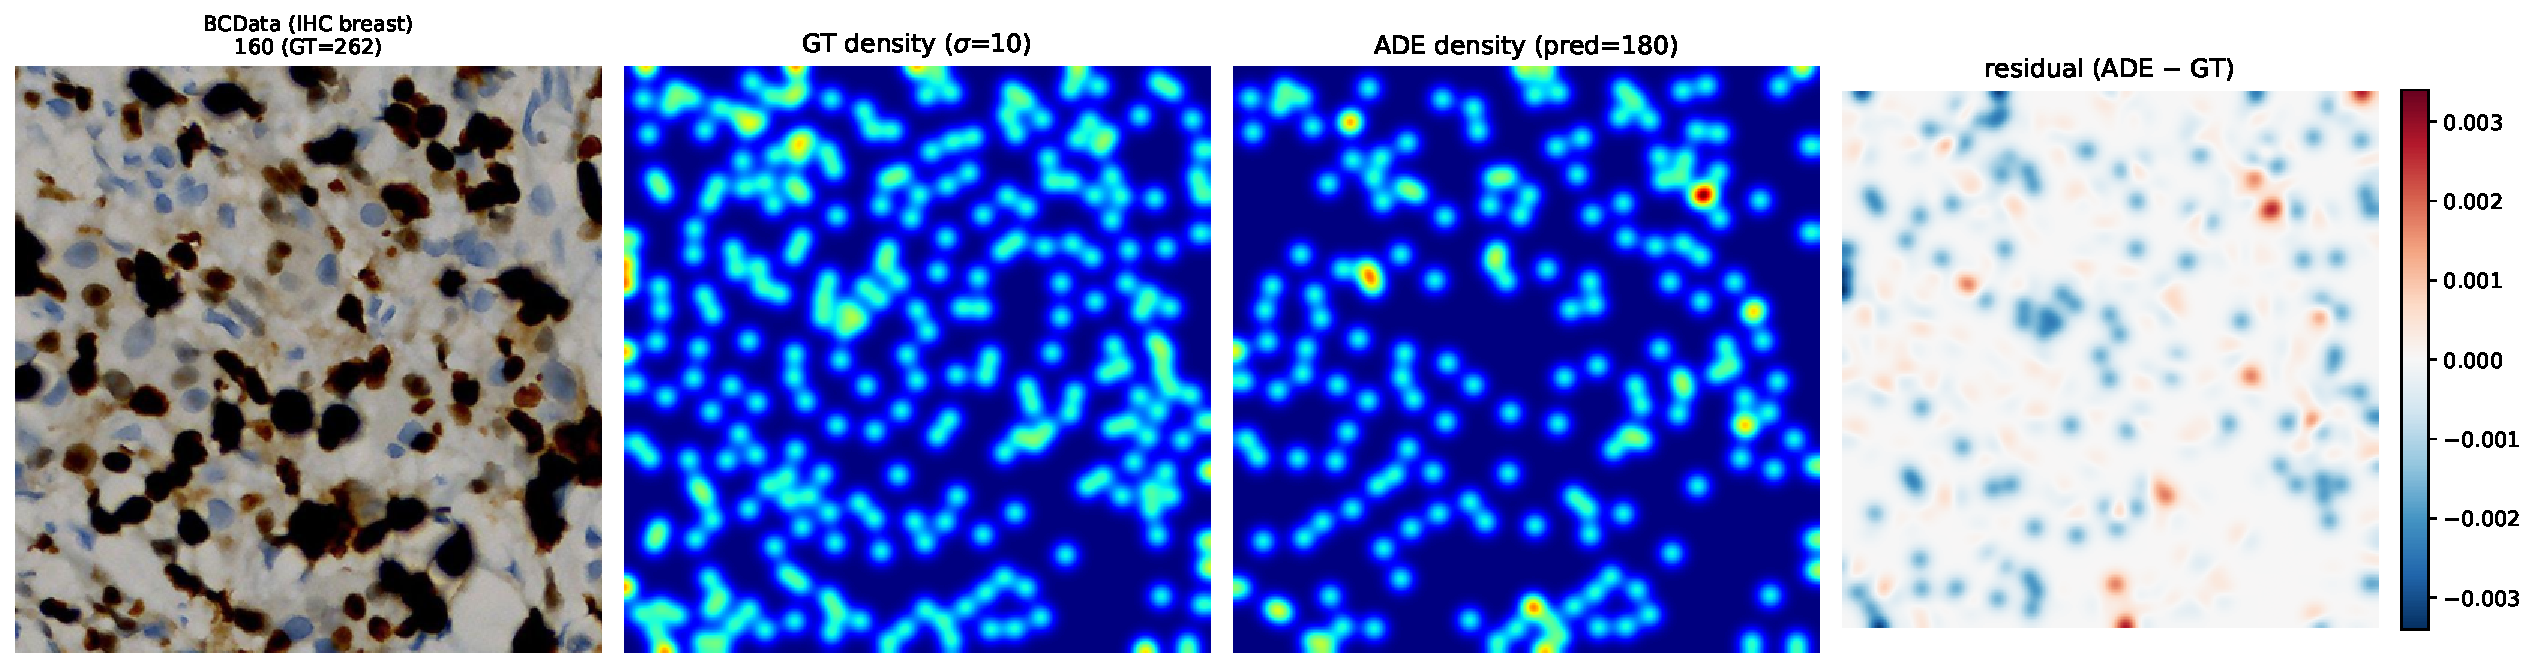
\includegraphics[width=\linewidth]{figures/fig_ADE_density_heatmap_BCData}
    \caption{密度热力图——BCData（样本 \texttt{160}，GT $262$，$\sigma{=}10$）。残差整体接近平衡，团块处有轻微起伏。}
    \label{fig:ADE-den-BCData}
\end{figure}

\begin{figure}[H]
    \centering
    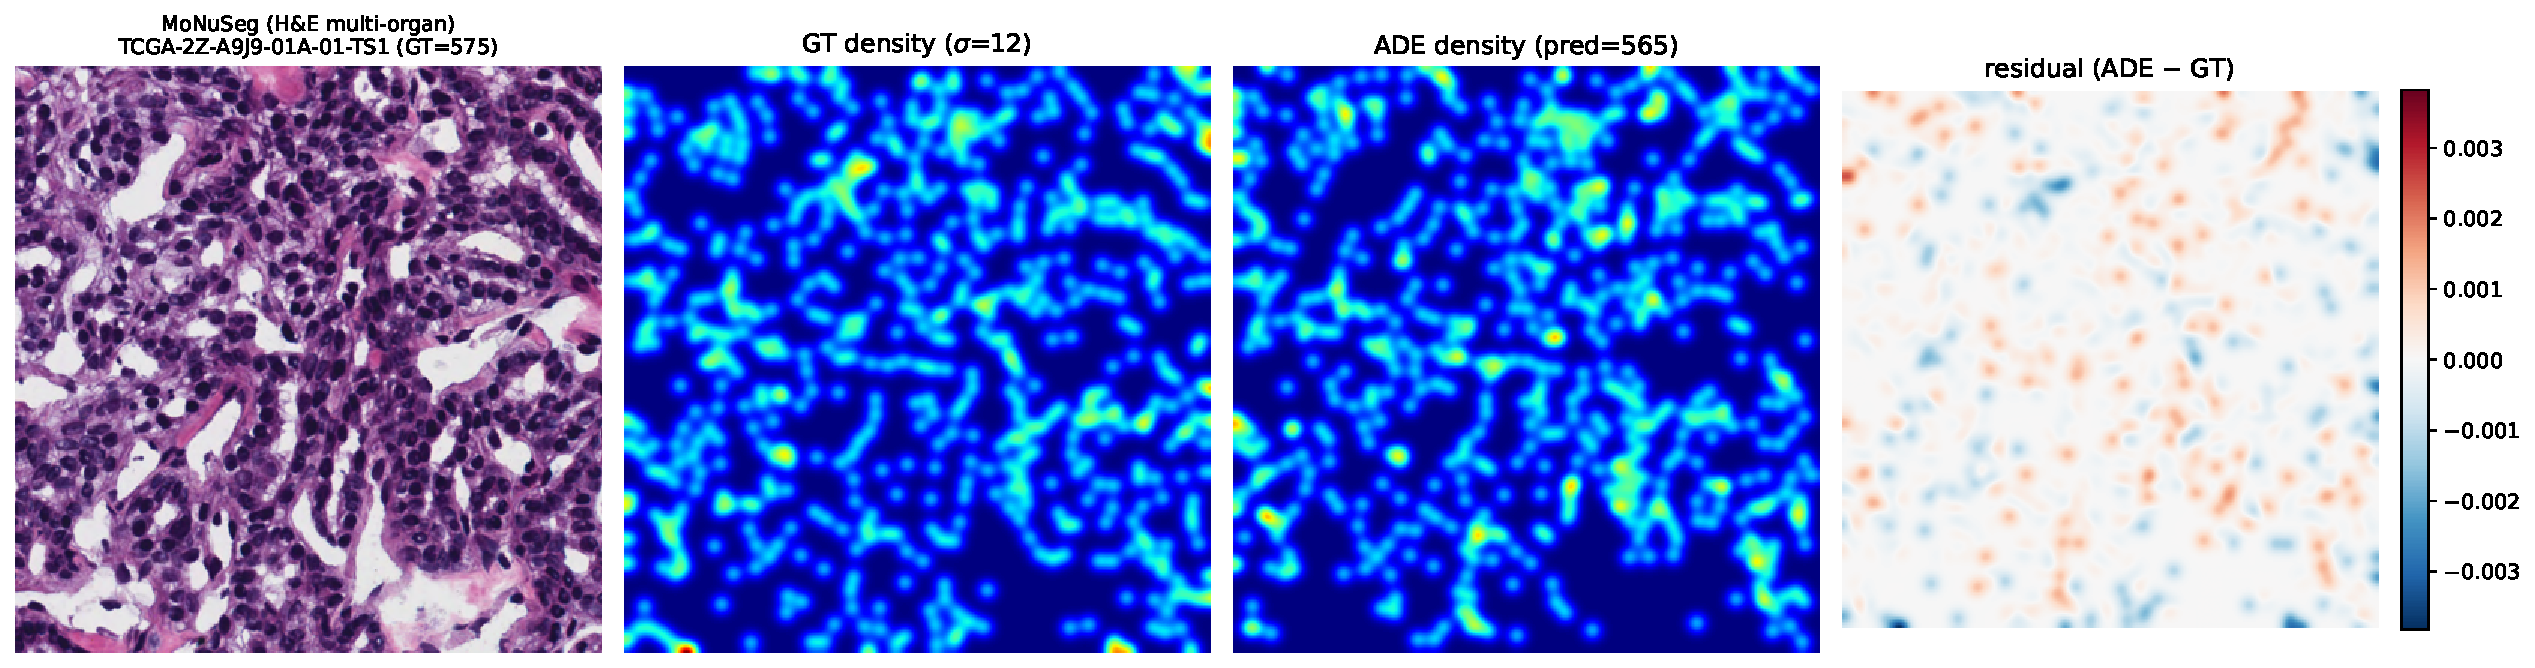
\includegraphics[width=\linewidth]{figures/fig_ADE_density_heatmap_MoNuSeg}
    \caption{密度热力图——MoNuSeg（\texttt{TCGA-2Z-A9J9-01A-01-TS1}，GT $575$，$\sigma{=}12$）。残差整体接近零，
    $0.5$ 处的过计已被阈值校准修正。}
    \label{fig:ADE-den-MoNuSeg}
\end{figure}

图~\ref{fig:ADE-reg-CoNIC}--\ref{fig:ADE-reg-MoNuSeg} 在 $4\times4$ 网格下给出区域级计数（GT、ADE 及偏差 $\Delta$、
逐区域误差热力图）以及\emph{全测试集}的计数误差--密度散点。三数据集的密度--误差散点均显示：低密度区 baseline 与
ADE 高度重合，而\emph{高密度区 baseline 大幅欠计（散点向下发散）、ADE 明显收敛回零线附近}——直观印证 ADE
（D 形变感受野 $+$ E 染色鲁棒）对"高密度少计"这一失败模式的针对性修复，尤以 CoNIC 最显著。

\begin{figure}[H]
    \centering
    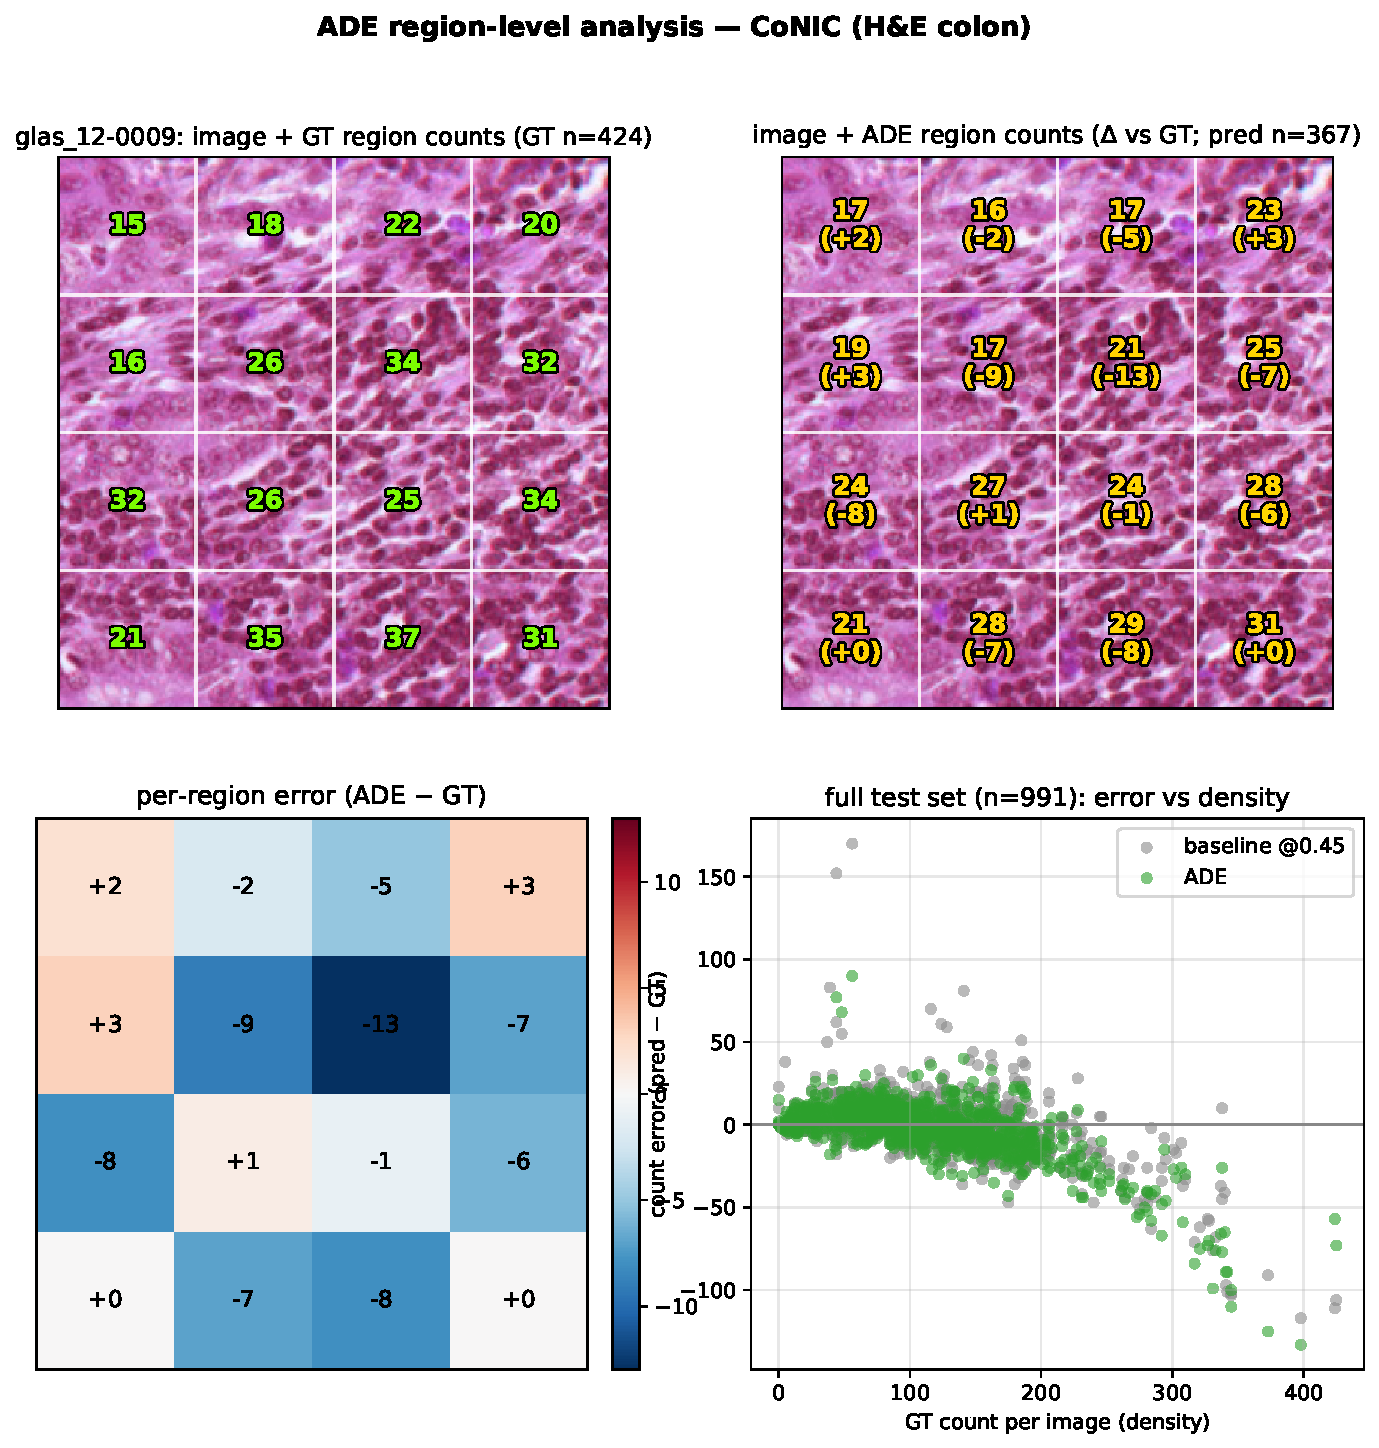
\includegraphics[width=\linewidth]{figures/fig_ADE_region_analysis_CoNIC}
    \caption{区域级分析——CoNIC（\texttt{glas\_12-0009}）。左上：\emph{原图}叠 $4\times4$ 网格与各区 GT 计数；
    右上：\emph{原图}叠网格与 ADE 各区计数（括号为与 GT 偏差 $\Delta$）；左下：逐区域误差（ADE$-$GT）热力图；
    右下：全测试集（$n{=}991$）计数误差--密度散点（灰 baseline、绿 ADE）。高密度区 ADE 明显收敛回零线。}
    \label{fig:ADE-reg-CoNIC}
\end{figure}

\begin{figure}[H]
    \centering
    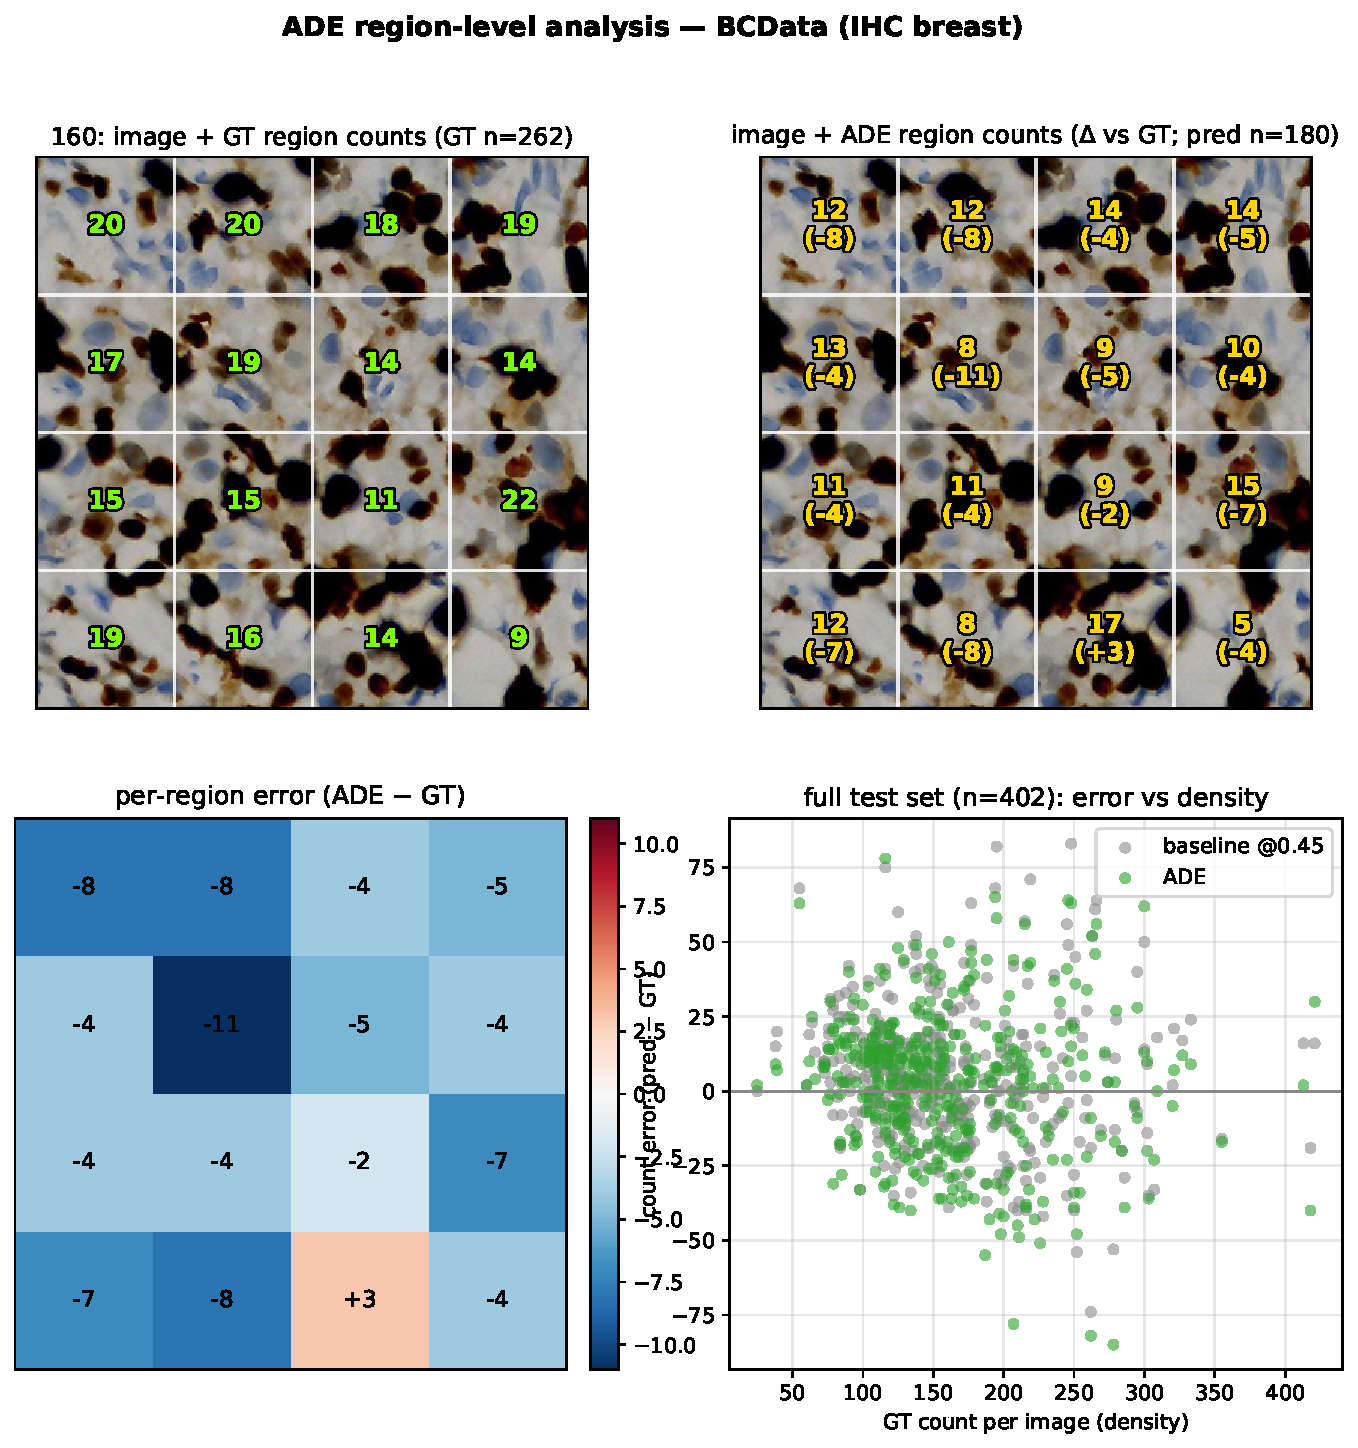
\includegraphics[width=\linewidth]{figures/fig_ADE_region_analysis_BCData}
    \caption{区域级分析——BCData（样本 \texttt{160}）。子图排布同上，散点基于全测试集 $402$ 张。低密度区两模型接近，
    ADE 在中高密度区略优。}
    \label{fig:ADE-reg-BCData}
\end{figure}

\begin{figure}[H]
    \centering
    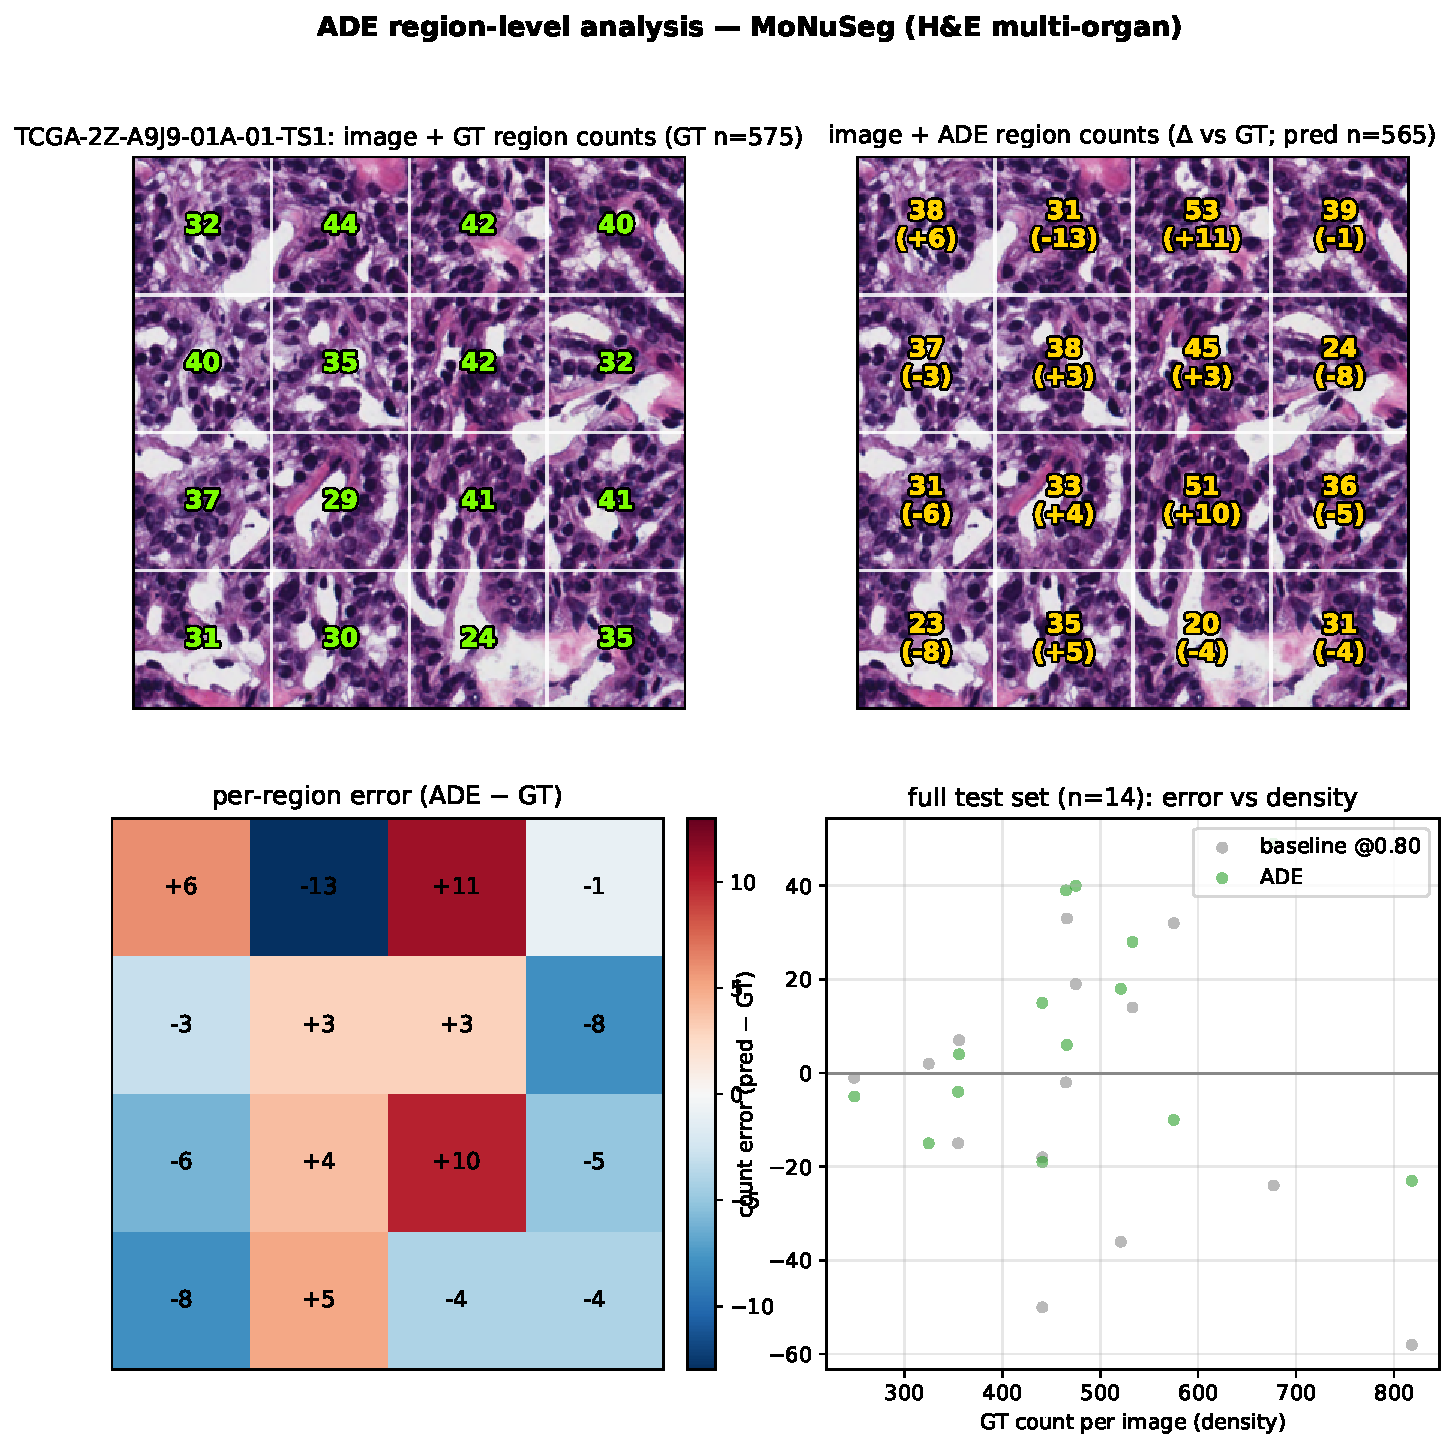
\includegraphics[width=\linewidth]{figures/fig_ADE_region_analysis_MoNuSeg}
    \caption{区域级分析——MoNuSeg（\texttt{TCGA-2Z-A9J9-01A-01-TS1}）。子图排布同上，散点基于全测试集 $14$ 张。
    ADE 计数误差整体更贴近零线（计数更准），但注意其定位 F1 低于 baseline。}
    \label{fig:ADE-reg-MoNuSeg}
\end{figure}

\paragraph{关键洞察（更正）：密度自适应后处理的"增益"是测试集调参的假象}
早前版本报告 A 的密度自适应在 D+E clean 上带来 $\Delta{=}{+}1.0$（$11.37\!\to\!10.37$）的增益，并据此得出
"后处理校准依赖基座标定质量"的结论。复核发现该数字\emph{不成立}：其分档阈值是用\emph{测试集}的 $2$-fold CV
选出的，等价于看着测试标签调超参，不是合法协议。改为正确的 val$\to$test（val 拟合分档边界与每档阈值、
冻结后套 test）后，密度分档 MAE 为 $12.27$，反而\emph{劣于}单一 val 全局阈值 $11.87$（$\Delta{=}{-}0.39$）；
且 val 与 test 上选出的分档阈值方向相反（$0.4/0.45/0.5$ vs $0.5/0.3/0.1$），说明"按密度分档"的信号在本任务上
不稳定、不可迁移。因此\emph{诚实的结论是}：ADE 在 CoNIC 上的净正收益来自 D+E 的结构改进，A 的密度自适应
后处理并无可靠增益——这也是一次关于"评测协议本身比数字更重要"的教训。

\paragraph{小结}
ADE 集成真正 net-positive 的形态是 \textbf{"D+E 结构改进 $+$ A 密度自适应后处理"}，但其收益\emph{对症于"高密度少计"}：
在设计靶点 CoNIC 上取得 MAE $10.37$、F1@12 $0.797$，计数与定位均优于 baseline；迁移到 BCData（与 baseline 持平略逊）
与 MoNuSeg（计数更好但定位更差）则得失参半，说明 D/E 的结构改进对形态/染色差异更大的数据集并非无条件收益。
与此同时，A 的激进训练配方（EOS$\downarrow$$+$focal）在 native 好基座上有害、应关闭，A 的价值应落在\emph{后处理校准}。
另一条稳健的工程结论是：\emph{小/IHC 数据集必须做阈值校准}——固定 $0.5$ 会因严重过计给出误导性指标，阈值选择的
影响甚至超过模型架构本身。

% =============================================================================
% BDC 集成框架 (由负责人填写)
% =============================================================================
\subsubsection{BDC 集成}

\paragraph{集成动机与组合逻辑。}对应困难样本诊断中的"密集漏检"与"粘连重复"两类问题：B 以密集辅助监督
提升高密度区召回、D 以形变卷积与边缘截断处理增强形态/边界鲁棒性、C 以点级排斥与密度自适应去重抑制
重复点。三者分别作用于\emph{监督信号、网络结构、后处理}，预期在密集粘连场景（CoNIC/MoNuSeg）形成互补。% TODO: 补充组合次序与预期.
待补充。

\paragraph{实现与配置。}% TODO: B 的 dense 分支 + D 的 DCNv2/Edge + C 的 Repulsion/Adaptive NMS 如何叠加; 训练与后处理流程; 数据集与划分.
待补充。

\paragraph{实验结果。}% TODO: 与 baseline、各单方向、以及 ADE 的对比; 计数 MAE/MSE 与定位 F1@6/12/24.
待补充。

\begin{table}[H]
    \centering
    \caption{BDC 集成结果（待填）}
    \label{tab:BDC-main}
    \small
    \begin{tabular}{lccccc}
        \toprule
        方法设置 & MAE$\downarrow$ & MSE$\downarrow$ & Recall$\uparrow$ & F1@12$\uparrow$ & 备注 \\
        \midrule
        APGCC baseline       & 待补充 & 待补充 & 待补充 & 待补充 & 待补充 \\
        B + D（结构）         & 待补充 & 待补充 & 待补充 & 待补充 & 待补充 \\
        B + D + C（完整 BDC） & 待补充 & 待补充 & 待补充 & 待补充 & 待补充 \\
        \bottomrule
    \end{tabular}
\end{table}

\paragraph{小结。}% TODO: BDC 的 net-positive 形态、各组件叠加是否互补或冲突、与 ADE 的适用场景差异.
待补充。
